\subsection{Loads and boundary conditions}

Both specimen ends are clamped in the test fixture. The tensile experiments are strain-controlled by means of a constant velocity on one of the clamping regions. The homogeneous displacement and inhomogeneous velocity boundary conditions are applied on respective node sets at the specimen ends. As these sets are defined on the base FE mesh, there is a small deviation of the application region in the PD model. This has no effect on the results. Various combinations of displacement boundary conditions were investigated. The influence on the results is negligible.

% BC:

\begin{figure}[htbp]
  \begin{subfigure}{0.49\linewidth}
    \centering
    %\includegraphics[width=\linewidth,height=4cm,keepaspectratio]{../../Material/Figures/Model_Mix_Hex_0-4_BC_NodeSets_Iso_ct}
    \includegraphics[width=\linewidth,height=4cm,keepaspectratio]{Model_Mix_Hex_0-4_BC_NodeSets_Iso_ct}
    \caption{Iso view}
    \label{fig:Model:Discretization:LBC:Iso}
  \end{subfigure}%
  \hfill
  \begin{subfigure}{0.49\linewidth}
    \centering
    %\includegraphics[width=\linewidth,height=4cm,keepaspectratio]{../../Material/Figures/Model_Mix_Hex_0-4_BC_NodeSets_ct}
    \includegraphics[width=\linewidth,height=4cm,keepaspectratio]{Model_Mix_Hex_0-4_BC_NodeSets_ct}
    \caption{Detail of FE (blue) and PD (green) node set}
    \label{fig:Model:Discretization:LBC:Detail}
  \end{subfigure}%
  \caption{Constraint and load introduction domains}
  \label{fig:Model:Discretization:LBC:Tet}
\end{figure}

% Boundary conditions: \cite{MadenciE2016} f�r ``richtige'' Randbedingungen nicht angewendet, aber Bereich Randbedingungen weit genug weg, sodass kein Einfluss R�nder auf Versagen

Madenci and Oterkus \cite{MadenciE2016} point out, that simply imposing constant boundary condition values on a material regions leads to incorrect behavior of the actual boundary and the domain within a distance of one horizon from the application region. A modified approach to reflect the correct boundary conditions is proposed but not used here as the no-failure-zone in the model is large enough to smooth boundary effects.

% \FloatBarrier